\section{Progettazione Concettuale : il Modello ER}
\subsection{Cos'è il modello ER}
Il \textbf{modello Entità-Relazione (ER)} è un linguaggio visivo usato per 
rappresentare i dati e comprendere come essi siano collegati tra loro. 
Viene utilizzato soprattutto nella fase iniziale di progettazione di un database, 
per avere un'idea chiara di quali informazioni siano necessarie e di come esse siano 
organizzate.
Esso è un linguaggio formale e non ambiguo.

\subsection{Costrutti del modello ER}
Gli strumenti fondamentali del modello ER vengono definiti come \textbf{costrutti}.
Ogni costrutto viene descritto specificando:
\begin{itemize}
    \item il \textbf{significato};
    \item la \textbf{sintassi grafica};
    \item la \textbf{rappresentazione delle sue istanze}.
\end{itemize}

\begin{tcolorbox}[colback=yellow!20!white, colframe=black, title=Cos'è un'istanza]
Un’\textbf{istanza} è un singolo elemento concreto che appartiene a un'entità.  

\begin{itemize}
    \item L’\textbf{entità} descrive il concetto generale (es. \emph{Studente});  
    \item L’\textbf{istanza} è un esempio reale di quell’entità (es. \emph{Mario Rossi}, matricola S123).  
\end{itemize}

\textbf{Esempio:}  
\begin{itemize}
    \item Entità: \emph{Studente} → attributi: matricola, nome, cognome;  
    \item Istanza: \{Matricola: S123, Nome: Luca, Cognome: Rossi\}.  
\end{itemize}

In sintesi: l’entità è il modello generale, mentre l’istanza è un caso reale e specifico di quell’entità.
\end{tcolorbox}

\subsection{Entità}
\begin{itemize}
    \item \textbf{Significato}: un’entità $E$ rappresenta una classe di oggetti
con le seguenti caratteristiche:
    \begin{itemize}
        \item hanno proprietà comuni;
        \item hanno esistenza autonoma;
        \item hanno identificazione univoca (esiste una
        chiara corrispondenza tra gli oggetti istanze
        di $E$ e i concetti istanziati nel sistema
        informativo).
    \end{itemize}

    \item \textbf{Sintassi grafica}: un’entità $E$ si rappresenta nello schema con
    un rettangolo che contiene il nome
    dell’entità.

    \item \textbf{Istanza}: un’istanza dell’entità $E$ è un oggetto
    appartenente alla classe rappresentata da $E$.
    Si indica con $I(E)$ l’insieme delle istanze di $E$ che
    esistono nella base di dati in un certo istante.
    (come definito nel riquadro precedente).

    \item \textbf{Esempio}: rappresento con il costrutto entità il concetto di
    \texttt{PERSONA}, ipotizzando che nei requisiti sia
    indicata la necessità di gestire nella base di dati le
    informazioni che descrivono un gruppo di
    persone e che tali informazioni possiedano nel
    sistema informativo le caratteristiche indicate
    nella semantica del costrutto entità.
\end{itemize}
    \begin{figure}[!h]
        \centering
        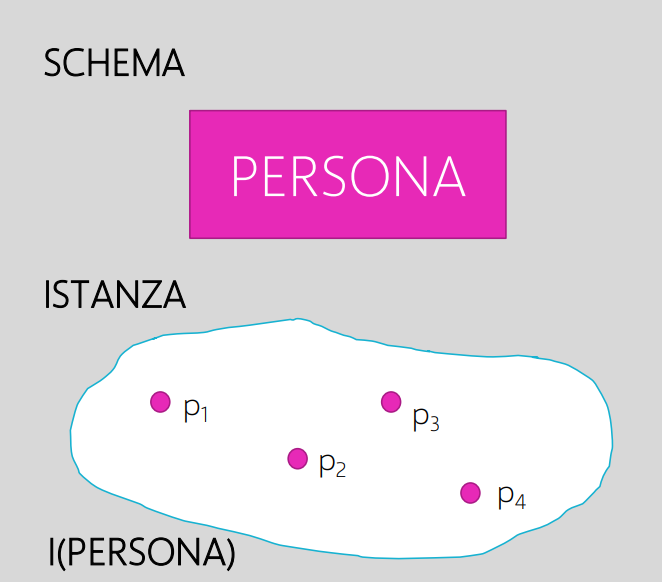
\includegraphics[width=0.5\linewidth]{image3.png}
        \caption{Esempio di Entita}
        \label{fig:placeholder}
    \end{figure}
\subsection{Relazione}
\begin{itemize}
    \item \textbf{Significato}: una relazione $R$ rappresenta un \textbf{legame logico} tra
    due o più entità.  
    Possono esistere relazioni:
    \begin{itemize}
        \item \textbf{binarie}, quando coinvolgono due entità diverse;
        \item \textbf{ternarie}, quando coinvolgono tre entità;
        \item \textbf{ennarie}, quando coinvolgono $n$ entità.  
    \end{itemize}
    \textbf{Caso particolare:} una relazione binaria può essere definita anche sulla stessa entità (detta \textbf{relazione ricorsiva}), ad esempio la relazione \emph{“impiegato-supervisore”} all’interno dell’entità \emph{Dipendente}.

    \item \textbf{Sintassi grafica}: una relazione $R$ si rappresenta nello schema
    con un \textbf{rombo} collegato, tramite linee spezzate, alle entità coinvolte nella
    relazione.  
    Il nome della relazione viene scritto all’interno o accanto al rombo.

    \item \textbf{Istanza}: data una relazione $R$ tra $n$ entità $E_1, E_2, \ldots, E_n$, 
    un’istanza della relazione è una \textbf{ennupla} di istanze delle entità coinvolte.  
    L’insieme di tutte le ennuple costituisce la \textbf{popolazione della relazione}.

    In altre parole, le ennuple rappresentano i \textbf{collegamenti concreti} tra le istanze delle entità.  
    Se immaginiamo la relazione come una tabella, ciascuna riga (ennupla) contiene i riferimenti alle istanze delle due entità collegate.  

    \textbf{Esempio:}  
    Sia $E =$ \emph{Studente} e $F =$ \emph{Corso}, e sia $R =$ \emph{Iscrizione}.  
    Un’istanza della relazione può essere l’ennupla $(\text{Mario Rossi}, \text{Analisi 1})$, 
    che rappresenta il fatto che lo studente “Mario Rossi” è iscritto al corso “Analisi 1”.  
    L’insieme di tutte le ennuple del tipo $(\text{Studente}, \text{Corso})$ forma la popolazione della relazione \emph{Iscrizione}.
    \item \textbf{Esempio} : Supponiamo di aver inserito nello schema le entità
\emph{PERSONA} e \emph{COMUNE}, e ipotizziamo che nei
requisiti sia indicata la necessità di gestire la
\emph{RESIDENZA} delle persone nei comuni italiani.
Rappresento con il costrutto relazione il concetto
di \emph{RESIDENZA}
\end{itemize}
\begin{figure}[!h]
    \centering
    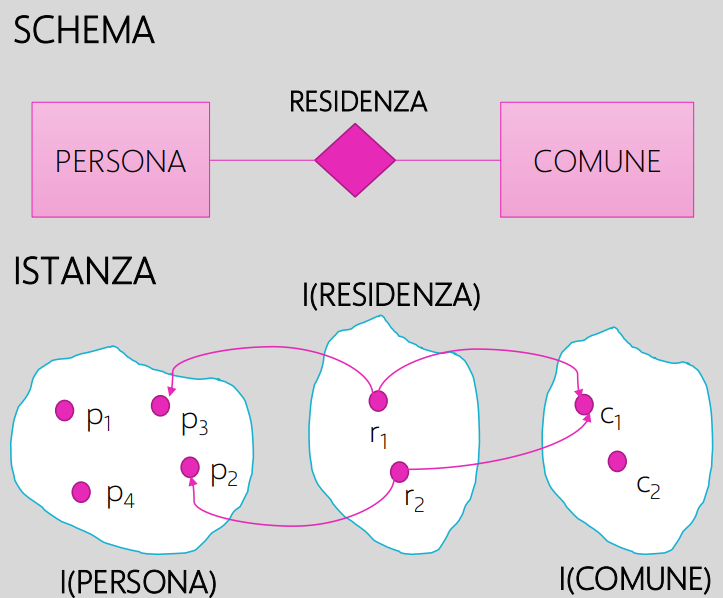
\includegraphics[width=0.5\linewidth]{image4.png}
    \caption{Esempio di Relazione}
    \label{fig:placeholder}
\end{figure}
\newpage
\subsubsection{Relazione Ricorsiva}
E’ una relazione binaria sulla stessa entità.
\begin{figure}[!h]
    \centering
    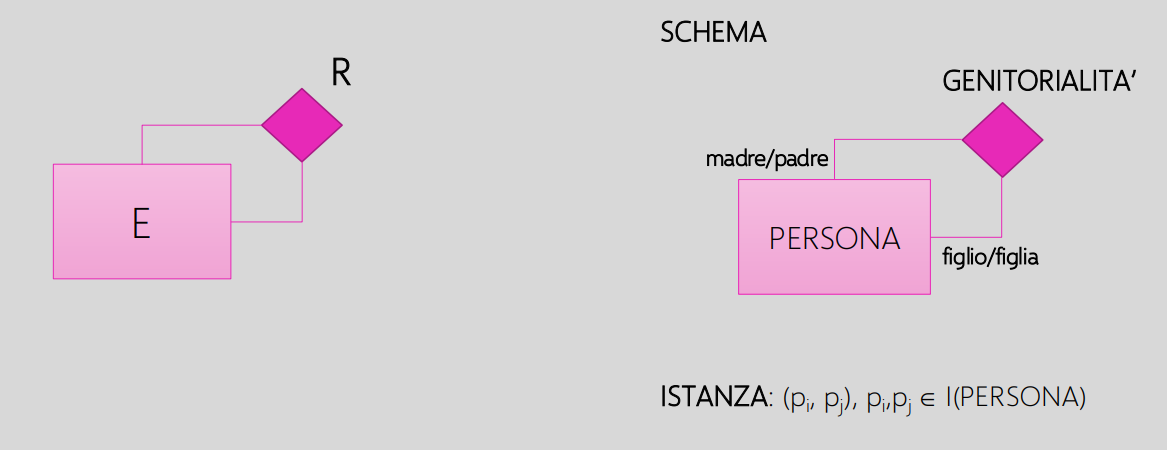
\includegraphics[width=0.7\linewidth]{image5.png}
    \caption{Relazione Ricorsiva}
    \label{fig:placeholder}
\end{figure}
\subsubsection{Relazione Ternaria}

Una \textbf{relazione ternaria} coinvolge tre entità e viene utilizzata quando un concetto del sistema informativo può essere rappresentato solo se sono presenti contemporaneamente tre istanze, una per ciascuna entità coinvolta.

\begin{itemize}
    \item Ogni istanza della relazione associa \textbf{una terna} di entità (E$_1$, E$_2$, E$_3$).  
    \item L’esistenza della relazione \textbf{richiede sempre} la presenza di tutte e tre le entità: non è possibile che ne manchi una.  
    \item Non esistono casi in cui la stessa terna debba essere rappresentata più volte.  
\end{itemize}

\begin{center}
    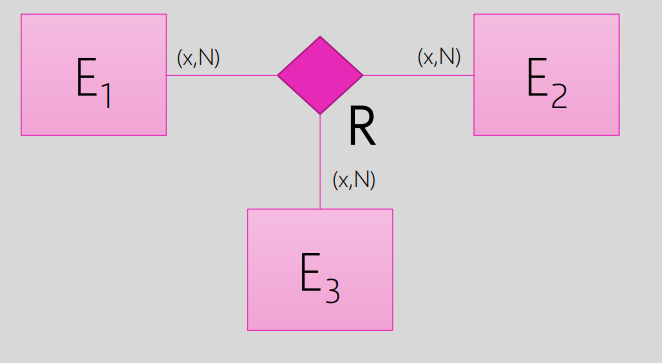
\includegraphics[width=0.55\linewidth]{image17.png}
    \label{fig:relazione_ternaria}
\end{center}

\subsubsection{Indizi di modellazione errata (uso improprio della relazione ternaria)}

In alcuni casi, l'utilizzo di una \textbf{relazione ternaria} può indicare una modellazione errata.  
Questo avviene quando una relazione tra tre entità non richiede realmente la presenza simultanea di tutte e tre le istanze.

\begin{itemize}
    \item Se per rappresentare lo stato del sistema informativo sarebbe sufficiente collegare \textbf{solo due entità per volta}, la relazione ternaria è superflua.  
    \item In tali casi, la relazione ternaria può essere sostituita da \textbf{tre relazioni binarie indipendenti}.
\end{itemize}



\noindent
\textbf{Esempio:}  
La relazione ternaria \emph{Partecipa(Medico, Paziente, Ospedale)} è errata se nel sistema esistono già le relazioni binarie:  
\emph{Lavora\_in(Medico, Ospedale)}, \emph{Visita(Medico, Paziente)} e \emph{Ricoverato\_in(Paziente, Ospedale)}.  
In questo caso, la relazione ternaria non aggiunge alcuna informazione nuova ed è quindi ridondante.
\noindent
Un ulteriore indizio di modellazione errata si verifica quando, in una relazione ternaria $R(A, B, C)$, si osserva il seguente comportamento:

\begin{itemize}
    \item Se una coppia $(a,b)$ compare in una terna $(a,b,c)$ istanza della relazione,  
    \item e una coppia $(b,c')$ compare in una terna $(a',b,c')$ istanza della relazione,
\end{itemize}

allora risultano automaticamente presenti anche le terne $(a,b,c')$ e $(a',b,c)$.

\noindent
Questo significa che le combinazioni tra le entità non dipendono realmente tutte e tre tra loro:  
la relazione ternaria può quindi essere scomposta in più relazioni binarie indipendenti senza perdita di informazione.
\noindent
\textbf{In sintesi:} se da due terne si possono dedurre automaticamente altre combinazioni tra le stesse entità,  
la relazione ternaria è ridondante e andrebbe sostituita da più relazioni binarie.

\begin{tcolorbox}[colback=yellow!15!white, colframe=orange!80!black, title=\textbf{Kristian semplifica in questo modo}]
Le \textbf{relazioni ternarie} vanno usate solo quando il significato della relazione dipende \textbf{strettamente da tutte e tre le entità coinvolte}.  

\begin{itemize}
    \item Se anche una sola entità può essere esclusa o rappresentata separatamente, allora la relazione non è veramente ternaria.  
    \item Nella maggior parte dei casi, è meglio sostituire una relazione ternaria con \textbf{più relazioni binarie indipendenti}.
\end{itemize}

\noindent
\textbf{In sintesi:}  
se puoi evitarla, \textbf{evitala}. Le relazioni ternarie rendono più difficile la progettazione e la traduzione nel modello relazionale.
\end{tcolorbox}
\subsubsection{Esempio coretto di relazione ternaria}
Vogliamo rappresentare il fatto che un prodotto venga fornito ad un dipartimento da un fornitore. Ogni
dipartimento può scegliere quali prodotti ordinare dai fornitori selezionando un sottoinsieme dei prodotti
forniti dal fornitore. Ogni fornitore vende a più dipartimenti prodotti diversi. Ogni prodotto viene venduto
da più fornitori.
\begin{figure}[!h]
    \centering
    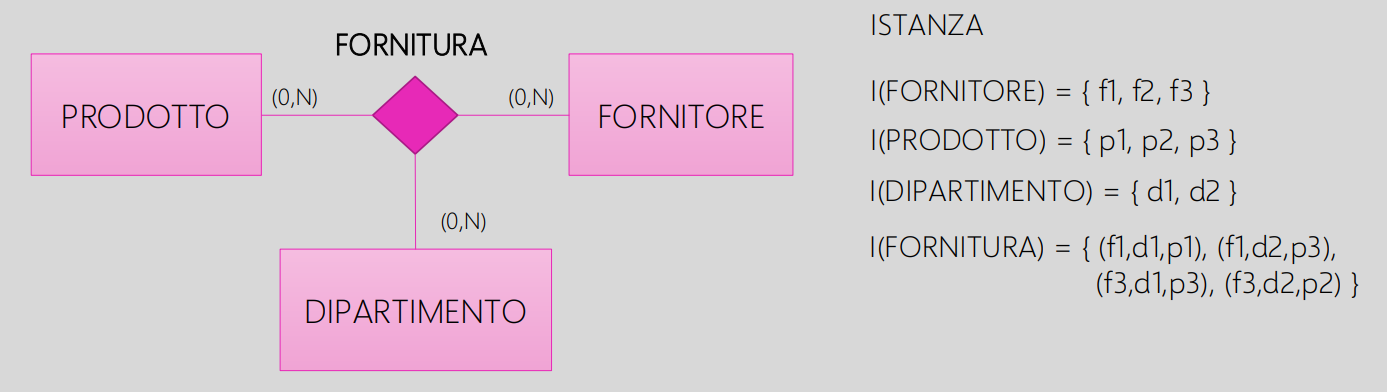
\includegraphics[width=0.75\linewidth]{image18.png}
    \caption{Esempio Relazione Ternaria}
    \label{fig:placeholder}
\end{figure}
\subsubsection{Come capire se un concetto ha vita propria}
Nel modello Entità-Relazione, per stabilire se un concetto debba essere rappresentato come 
\textbf{entità} o come \textbf{relazione}, è fondamentale chiedersi se tale concetto
\textit{ha una vita propria} all'interno del sistema informativo.

\begin{tcolorbox}[colback=yellow!15!white, colframe=black, title=Definizione]
Un concetto ha \textbf{vita propria} se può esistere in modo indipendente dalle altre entità,
cioè se ha senso considerarlo come un oggetto autonomo, anche quando non è collegato ad altri.
\end{tcolorbox}

\noindent
Per verificarlo, è possibile porsi alcune domande:

\begin{itemize}
  \item Può esistere anche senza essere collegato ad altre entità?
  \item Ha senso registrarlo nel sistema anche se non è associato ad altri elementi?
  \item Possiede attributi che descrivono sé stesso e non il legame con altri?
\end{itemize}

\noindent
Se la risposta è \textbf{sì} a queste domande, il concetto possiede vita propria e deve essere rappresentato come \textbf{entità}.
In caso contrario, se esiste solo come collegamento tra altre entità, è più corretto rappresentarlo come \textbf{relazione}.

\begin{center}
\begin{tabular}{|p{3.2cm}|p{5.3cm}|p{5.3cm}|}
\hline
\textbf{Caratteristica} & \textbf{Entità (ha vita propria)} & \textbf{Relazione (non ha vita propria)} \\
\hline
Esiste indipendentemente da altre & Può esistere da sola nel sistema & Esiste solo se collega altre entità \\
\hline
Ha senso da sola & Ha significato anche isolata & Ha senso solo nel contesto di un legame \\
\hline
Attributi & Descrivono l’oggetto in sé & Descrivono il legame tra entità \\
\hline
Esempio & Studente, Insegnamento, Docente & Sostiene, Frequenta, Acquista \\
\hline
\end{tabular}
\end{center}

\noindent
\textbf{Esempio applicativo:} nel caso della relazione \textit{ESAME}, se essa rappresenta l'atto con cui
uno studente sostiene un insegnamento (registrando solo \textit{data} e \textit{voto}),
non ha vita propria e va modellata come \textbf{relazione}.
Se invece si vogliono gestire appelli d’esame con \textit{aula}, \textit{docente} e \textit{orario}, 
esso assume significato autonomo e può essere rappresentato come \textbf{entità}.





\subsection{Attributo}
\begin{itemize}
    \item \textbf{Significato} :Rappresenta una proprietà elementare di un’entità (o
relazione).
Ogni attributo di entità (o relazione) associa ad ogni
istanza di entità (o relazione) UNO e UN SOL valore
appartenente ad un dominio (insieme di VALORI
AMMISSIBILI). 
    \item \textbf{Sintassi grafica} : collegato a una entità e a forma di pallino
\item \textbf{Esempio} : Rappresento con il costrutto entità il concetto di
PERSONA, ipotizzando che nei requisiti sia indicata
la necessità di gestire nella base di dati il nome e il
cognome di un gruppo di persone.
Aggiungo quindi il nome e il cognome come
attributi dell’entità PERSONA.
\begin{figure}[!h]
    \centering
    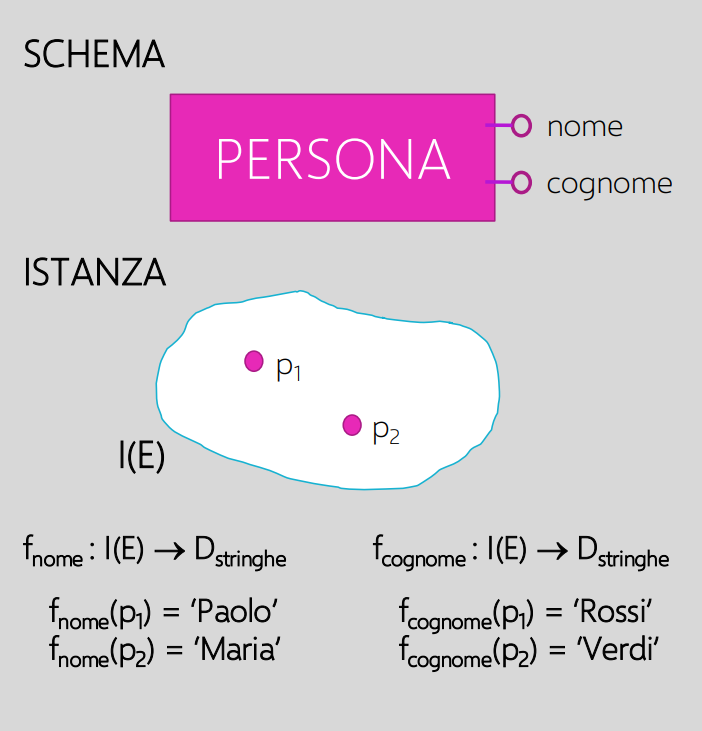
\includegraphics[width=0.5\linewidth]{image6.png}
    \caption{Esempio Attributo}
    \label{fig:placeholder}
\end{figure}
\subsubsection{Attributo opzionale e multivalore}  
Un \textbf{attributo opzionale} o \textbf{multivalore} deriva da un attributo normale, specificando un \textbf{vincolo di cardinalità} sui valori che esso può assumere.  
Il vincolo di cardinalità indica quante volte un attributo può comparire in corrispondenza di una stessa entità.  
Il valore predefinito è \textbf{(1,1)}, che significa “obbligatorio e singolo valore”.  

I principali casi sono:  
\begin{itemize}
    \item \textbf{(0,1)} : attributo opzionale → può essere assente o presente una sola volta;  
    \item \textbf{(1,N)} : attributo multivalore → deve essere presente almeno una volta e può comparire più volte;  
    \item \textbf{(0,N)} : attributo opzionale e multivalore → può essere assente o, se presente, avere più valori.
\end{itemize}

\begin{figure}[!h]
    \centering
    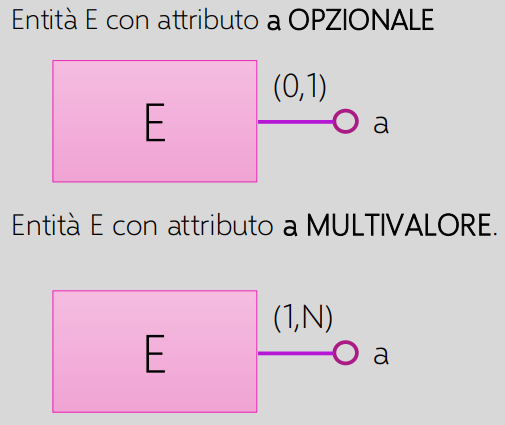
\includegraphics[width=0.5\linewidth]{image12.png}
    \caption{Attributo opzionale e/o multivalore}
    \label{fig:placeholder}
\end{figure}

\noindent
\textbf{Esempio pratico}  

Si consideri l’entità \emph{PERSONA}, per la quale si vogliono memorizzare:
\begin{itemize}
    \item \textbf{Codice fiscale}, \textbf{nome}, \textbf{cognome} e \textbf{data di nascita} — attributi obbligatori e a singolo valore;  
    \item \textbf{Patente di guida} — attributo \textbf{opzionale} \((0,1)\), poiché una persona può possederla o meno;  
    \item \textbf{Recapiti telefonici} — attributo \textbf{multivalore} \((1,N)\), poiché ogni persona può avere uno o più numeri di telefono (ad esempio cellulare, casa, lavoro).
\end{itemize}

\noindent


\begin{figure}[!h]
    \centering
    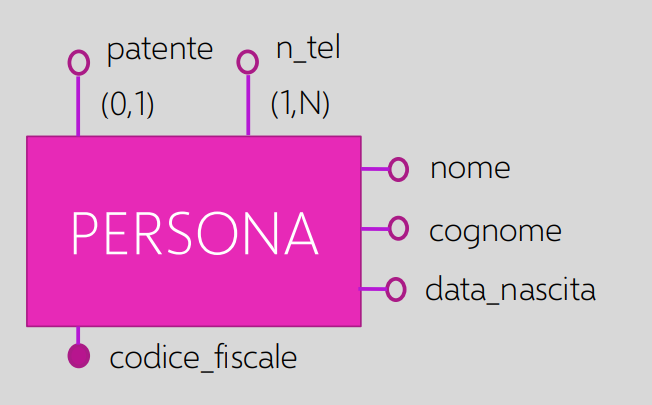
\includegraphics[width=0.5\linewidth]{image13.png}
    \caption{Esempio di attributo opzionale e multivalore per l’entità PERSONA}
    \label{fig:placeholder}
\end{figure}
\end{itemize}
\subsubsection{Attributo composto}
Un \textbf{attributo composto} consente di raggruppare più attributi di un’entità o di una relazione che presentano una stretta \textbf{affinità di significato}.  
In questo modo si possono rappresentare in modo più ordinato e logico informazioni che, pur essendo distinte, appartengono a un unico concetto complessivo.

\noindent
Ad esempio, per rappresentare l’entità \emph{PERSONA}, si possono gestire nella base di dati i seguenti attributi:  
\textbf{codice fiscale}, \textbf{nome}, \textbf{cognome}, \textbf{data di nascita} e \textbf{indirizzo}.  

\noindent
L’attributo \textbf{indirizzo} può essere considerato un attributo composto, poiché a sua volta può essere suddiviso nei sottoattributi:
\begin{itemize}
    \item \textbf{Città}
    \item \textbf{Via}
    \item \textbf{Numero civico}
\end{itemize}

\noindent
In un diagramma ER, l’attributo composto viene rappresentato con un’ellisse principale collegata a più ellissi minori, ognuna delle quali rappresenta un sottoattributo.

\begin{figure}[!h]
    \centering
    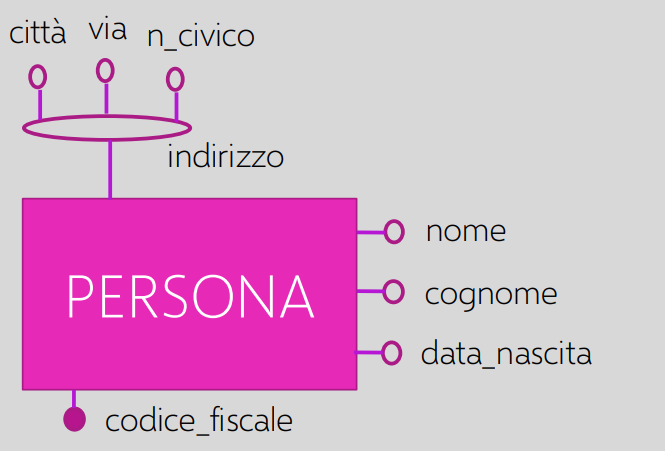
\includegraphics[width=0.5\linewidth]{image14.png}
    \caption{Esempio di attributo composto per l’entità PERSONA}
    \label{fig:placeholder}
\end{figure}


\subsection{Identificatore di Entità}
\begin{itemize}
    \item \textbf{Significato}:Data un’entità E, è un insieme di proprietà (attributi
e/o relazioni) che identificano univocamente le
istanze dell’entità.
Un insieme di proprietà \textbf{IDENTIFICA
UNIVOCAMENTE} le istanze di E se non esistono
due istanze di E che presentano gli stessi
valori/istanze nelle proprietà dell’insieme.
    \item \textbf{Sintassi grafica} : collegato a una entità e a forma di un pallino pieno, puo anche essere una linea che intercorre in due attributi sempre a fine con un pallino pieno
    \begin{figure}[!h]
        \centering
        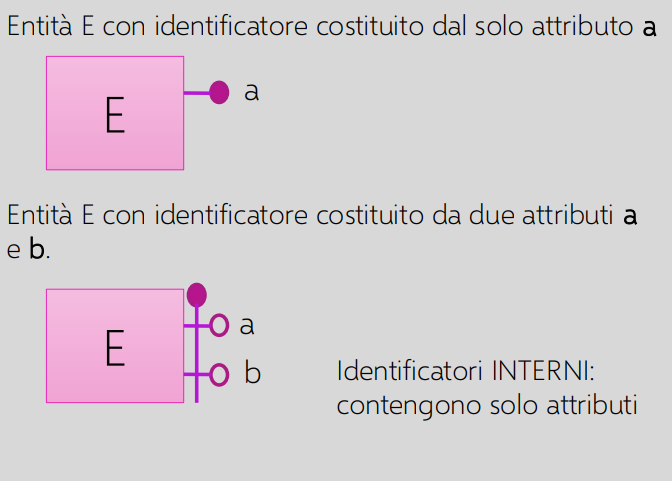
\includegraphics[width=0.5\linewidth]{image7.png}
        \caption{sintassi grafica: identificatori interni}
        \label{fig:placeholder}
    \end{figure}
    \begin{figure}[!h]
        \centering
        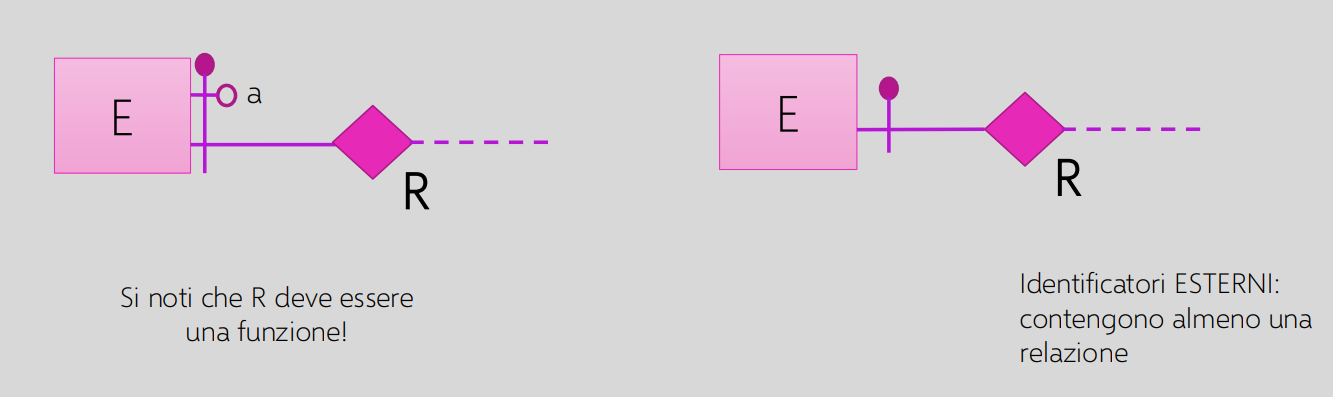
\includegraphics[width=0.75\linewidth]{image8.png}
        \caption{sintassi grafica: identificatori esterni}
        \label{fig:placeholder}
    \end{figure}
    \newpage
\item \textbf{Esempio}:
Rappresento con il costrutto entità il concetto di
\emph{PERSONA}, ipotizzando che nei requisiti sia indicata
la necessità di gestire nella base di dati, il codice
fiscale, il nome, il cognome e la data di nascita di un
gruppo di persone.
\begin{figure}[!h]
    \centering
    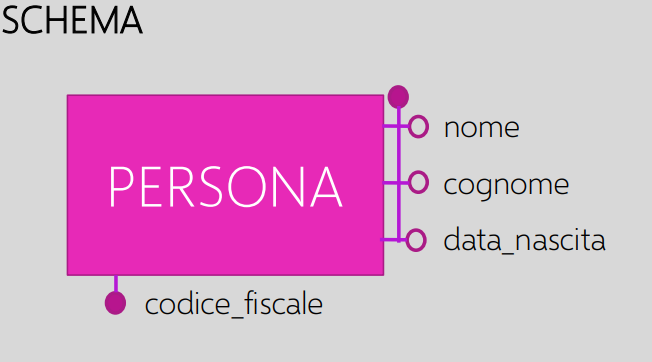
\includegraphics[width=0.5\linewidth]{image9.png}
    \label{fig:placeholder}
\end{figure}
\end{itemize}
La scelta dell’identificatore va sempre
fatta considerando proprietà
significative per il sistema informativo.
A livello concettuale l’introduzione di
nuovi attributi identificatori (ad
esempio l’ID) è da \textbf{evitare}.
\subsection{Generalizzazione}
La \textbf{generalizzazione} rappresenta un legame logico, analogo al concetto di \textbf{ereditarietà} nella programmazione a oggetti, tra un’entità padre e una o più entità figlie.  
Serve per modellare situazioni in cui più entità condividono alcune caratteristiche comuni, ma possiedono anche attributi o relazioni specifiche.

\begin{itemize}
    \item \textbf{Significato}:  
    È una relazione logica tra un’entità padre \emph{E} e $n$ entità figlie ($E_1, E_2, \ldots, E_n$), dove $E$ rappresenta una classe di oggetti più generale rispetto a quelle rappresentate dalle entità figlie.  
    Le entità figlie ereditano gli attributi e le relazioni dell’entità padre, aggiungendo eventualmente elementi propri.

    \item \textbf{Sintassi grafica}:  
    Le entità figlie coinvolte nella generalizzazione vengono collegate all’entità padre mediante una linea che converge in un triangolo (o freccia) rivolto verso l’entità padre.

    \begin{figure}[!h]
        \centering
        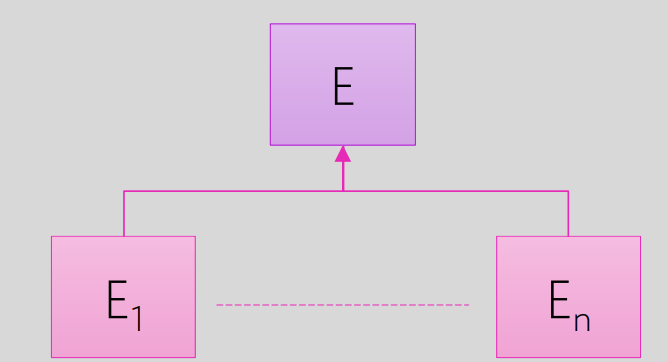
\includegraphics[width=0.5\linewidth]{image16.png}
        \caption{Sintassi grafica della generalizzazione}
        \label{fig:placeholder}
    \end{figure}

    \item \textbf{Esempio}:  
    Si consideri l’entità \emph{PERSONA}, per la quale nei requisiti è indicata la necessità di distinguere tra \emph{STUDENTE} e \emph{DOCENTE}.  
    In questo caso si può utilizzare una generalizzazione in cui:
    \begin{itemize}
        \item \textbf{PERSONA} è l’entità padre, che contiene gli attributi comuni (ad esempio: nome, cognome, data di nascita);
        \item \textbf{STUDENTE} e \textbf{DOCENTE} sono le entità figlie, che ereditano gli attributi di PERSONA e possono avere attributi propri (es. matricola per STUDENTE, dipartimento per DOCENTE).
    \end{itemize}

    \begin{figure}[!h]
        \centering
        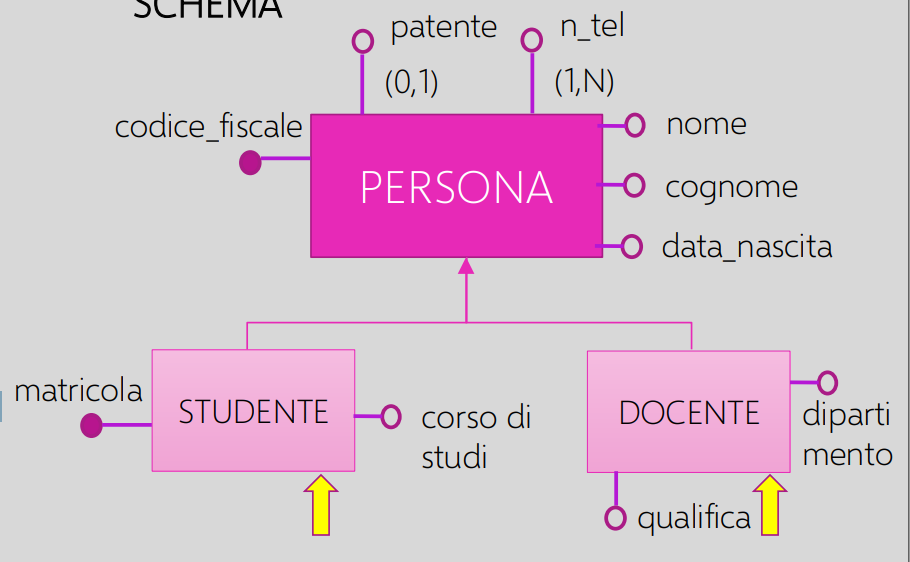
\includegraphics[width=0.5\linewidth]{image15.png}
        \caption{Esempio di generalizzazione tra PERSONA, STUDENTE e DOCENTE}
        \label{fig:placeholder}
    \end{figure}
\end{itemize}



\begin{tcolorbox}[colback=yellow!15!white, colframe=orange!80!black, title=\textbf{Proprietà}]
Le \textbf{proprietà delle istanze di entità} che partecipano a una \textbf{generalizzazione} sono le seguenti:

\begin{itemize}
    \item Ogni istanza di un’entità figlia $E_i$ è anche un’istanza dell’entità padre $E$.
    \item Ogni proprietà (attributi, identificatori e relazioni) dell’entità padre $E$ è condivisa da tutte le entità figlie $E_1, E_2, \ldots, E_n$.
\end{itemize}

\noindent
In altre parole, le entità figlie \textbf{ereditano} tutte le caratteristiche dell’entità padre, e possono aggiungerne di proprie.
\end{tcolorbox}
\subsubsection{Classificazione delle Generalizzazioni}
Nel modello \textbf{Entità–Relazione}, una generalizzazione può assumere diverse forme, a seconda del tipo di legame tra l’entità padre (superclasse) e le entità figlie (sottoclassi).  
Le combinazioni derivano dall’incrocio di due caratteristiche fondamentali:  
\begin{itemize}
    \item il grado di \textbf{copertura} (Totale o Parziale);  
    \item il grado di \textbf{esclusività} (Esclusiva o Sovrapposta).  
\end{itemize}

\noindent
Ecco i principali tipi di gerarchia nel modello ER:

\begin{enumerate}
    \item \textbf{Totale ed Esclusiva (t,e)}:  
    ogni istanza della superclasse appartiene \textbf{obbligatoriamente} a una e una sola sottoclasse.  
    \emph{Esempio:} l’entità \emph{VEICOLO} è generalizzata in \emph{MOTO} e \emph{AUTO}.  
    Ogni veicolo deve essere o moto o auto, ma non può essere entrambi.

    \item \textbf{Totale e Sovrapposta (t,s)}:  
    ogni istanza della superclasse deve appartenere ad almeno una sottoclasse, ma può appartenere a \textbf{più sottoclassi} contemporaneamente.  
    \emph{Esempio:} l’entità \emph{PERSONA} è generalizzata in \emph{STUDENTE} e \emph{LAVORATORE}.  
    Una persona può essere sia studente sia lavoratore.

    \item \textbf{Parziale ed Esclusiva (p,e)}:  
    non tutte le istanze della superclasse devono appartenere a una sottoclasse; se appartengono, ne hanno solo una.  
    \emph{Esempio:} l’entità \emph{ANIMALE} è generalizzata in \emph{DOMESTICO} e \emph{SELVATICO}.  
    Un animale può essere domestico, selvatico o nessuno dei due, ma non entrambi.

    \item \textbf{Parziale e Sovrapposta (p,s)}:  
    non tutte le istanze devono appartenere a una sottoclasse; chi appartiene può essere in più sottoclassi.  
    \emph{Esempio:} l’entità \emph{PERSONA} è generalizzata in \emph{SPORTIVO} e \emph{ARTISTA}.  
    Una persona può essere sportiva, artista, entrambe o nessuna delle due.
\end{enumerate}

\begin{tcolorbox}[colback=yellow!15!white, colframe=orange!80!black, title=\textbf{Kristian semplifica in questo modo}]
Le \textbf{gerarchie di generalizzazione} si classificano in base a due proprietà fondamentali:

\begin{itemize}
    \item \textbf{Totale} → ogni istanza della superclasse deve appartenere ad almeno una sottoclasse.  
    \item \textbf{Parziale} → alcune istanze della superclasse possono non appartenere a nessuna sottoclasse.  
    \item \textbf{Esclusiva (o Disgiunta)} → un’istanza può appartenere solo a una sottoclasse.  
    \item \textbf{Sovrapposta} → un’istanza può appartenere a più sottoclassi contemporaneamente.
\end{itemize}

\noindent
In sintesi:  
\textbf{Totale/Parziale} indica \emph{se tutte le istanze partecipano},  
mentre \textbf{Esclusiva/Sovrapposta} indica \emph{come partecipano}.
\end{tcolorbox}
